\section{Related Work}\label{sec:related}

\textbf{Vector quantization for ANN.}
Classical ANN compression methods such as Product Quantization (PQ)\slash OPQ~\cite{jegou2011pq,ge2013opq}
quantize vectors by subspace codebooks, while newer systems such as
ScaNN\slash SOAR\slash QAQ~\cite{guo2020scann,sun2023soar,zhang2023qaq} improve scoring,
routing, or query-aware ranking through anisotropic quantization and
query-dependent computation. In the 1-bit regime,
RaBitQ~\cite{gao2024rabitq} provides distortion bounds for BQ,
Extended-RaBitQ~\cite{gao2025extended} generalizes this line to multi-bit
settings, and later variants integrate quantization with graph
structures~\cite{gou2025symphonyqg}. Binary hashing methods such as
ITQ~\cite{gong2013itq} similarly rely on distributional alignment. Across
these lines, the standard assumption is that query and database statistics are
in-distribution and approximately centroid-aligned.

\textbf{Cross-modal and OOD retrieval.}
Cross-modal and OOD retrieval methods usually intervene outside compressed code formation.
OOD-DiskANN~\cite{jaiswal2022ood,subramanya2019diskann} augments
graph search for distribution shift; RoarGraph/DEG~\cite{chen2024roargraph,yin2025deg}
modify graph connectivity; DeDrift~\cite{baranchuk2023dedrift} and
TCR~\cite{li2025tcr} use test-time adaptation or retraining-style updates to
counter drift. They are effective but usually assume uncompressed vectors, additional graph
structures, or online serving updates. PMC is complementary, not a direct
baseline: one offline centroid correction in the 1-bit compressed regime, with
no added index-time memory or retraining.

\textbf{Modality gap.}
Mind-the-Gap~\cite{liang2022mind} shows that cross-modal embedding spaces often
exhibit stable centroid offsets between modalities. Follow-up analyses attribute
this behavior to training dynamics~\cite{schrodi2025twoeffects}, characterize
its geometry~\cite{levi2025doubleellipsoid}, and study mean-subtraction effects~\cite{zhang2024c3}.
Other work either preserves the gap~\cite{ramasinghe2024acceptgap} or reduces it
through encoder retraining~\cite{eslami2025alignclip}; see also the
recent survey~\cite{wang2024crossmodal}. No prior work addresses how the
modality gap degrades \emph{compressed} ANN indexes, where centroid
misalignment corrupts both IVF routing and quantized codes; this is our focus.

A closely related line, gap-aware calibration for mixed-modality ranking~\cite{li2025grclip}, rescales scores to offset the centroid gap but works on uncompressed vectors, never enters code formation, and still subtracts the query mean at query time; PMC instead folds the correction into the database index at $\alpha{=}1$, rewriting IVF routing and binary codes at the source with no serving-time query transform.

\begin{table}[t]
\caption{BQ methods (R@100, Vanilla\,/\,PMC) on MSCOCO (CLIP-B/32) and AudioCaps (IB). RotatedBinary\,=\,rotated BinaryFlat (BBQ-style).}\label{tab:signbit_methods}
\centering
{\small
\begin{tabular*}{\columnwidth}{@{\extracolsep{\fill}}l cc cc@{}}
\toprule
& \multicolumn{2}{c}{\textbf{MSCOCO}} & \multicolumn{2}{c}{\textbf{AudioCaps}} \\
\cmidrule(lr){2-3}\cmidrule(lr){4-5}
\textbf{Method} & t$\to$i & i$\to$t & t$\to$a & a$\to$t \\
\midrule
BinaryFlat    & .51\,/\,\textbf{.57} & .46\,/\,\textbf{.57} & .63\,/\,\textbf{.66} & .51\,/\,\textbf{.64} \\
BinaryIVF     & .51\,/\,\textbf{.57} & .47\,/\,\textbf{.57} & .59\,/\,\textbf{.61} & .50\,/\,\textbf{.63} \\
RotatedBinary & .29\,/\,\textbf{.58} & .21\,/\,\textbf{.57} & .65\,/\,\textbf{.70} & .63\,/\,\textbf{.69} \\
RaBitQ        & .58\,/\,\textbf{.64} & .52\,/\,\textbf{.61} & \textbf{.75}\,/\,\textbf{.75} & .67\,/\,\textbf{.75} \\
\bottomrule
\end{tabular*}
}
\end{table}

\begin{figure}[t]
\nointerlineskip\hrule height 0.8pt\vspace{1pt}%
{\setlength{\abovecaptionskip}{0pt}\setlength{\belowcaptionskip}{0pt}%
\captionsetup{justification=raggedright,singlelinecheck=false}%
\captionof{algorithm}{PMC Index Construction}\label{alg:pmc}}%
\vspace{1pt}\nointerlineskip\hrule height 0.4pt\vspace{1pt}%
\footnotesize
\begin{algorithmic}[1]
\Require Database $\mathcal{X}$ (modality~$b$), query sample $\mathcal{Q}$ (modality~$a$), interpolation $\alpha$
\Ensure IVF-based quantized index $\mathcal{I}$ and gap $\mathbf{g}$
\State $\boldsymbol{\mu}_q \gets \mathrm{mean}(\mathcal{Q})$; \quad $\boldsymbol{\mu}_x \gets \mathrm{mean}(\mathcal{X})$
\State $\mathbf{g} \gets \boldsymbol{\mu}_q - \boldsymbol{\mu}_x$
\For{each $\mathbf{x} \in \mathcal{X}$}
  \State $\mathbf{x}' \gets \mathrm{normalize}(\mathbf{x} + \alpha \, \mathbf{g})$
\EndFor
\State $\mathcal{I} \gets \mathrm{BuildIndex}(\{\mathbf{x}'\})$ \Comment{RaBitQ, BBQ, BinaryFlat}
\State \Return $\mathcal{I}$, $\mathbf{g}$
\end{algorithmic}%
\nointerlineskip\hrule height 0.8pt
\Description{Pseudocode for PMC index construction: compute modality means and gap, shift each database vector by alpha times the gap, normalize, then build the quantized index.}
\end{figure}

\begin{table*}[t]
\caption{PMC main retrieval results (R@100, $\alpha{=}1$, IVFRaBitQFastScan) at the two operating points of Sec.~\ref{sec:exp-setup}: \emph{No reranking} and \emph{With reranking}. Each cell Vanilla\,/\,MeanShift\,/\,PMC; \textbf{bold}\,=\,best per cell.}\label{tab:mainresults}
\centering
{\small
\begin{tabular*}{\textwidth}{@{\extracolsep{\fill}}llc ccc ccc@{}}
\toprule
 & & & \multicolumn{3}{c}{\textbf{No reranking}} & \multicolumn{3}{c}{\textbf{With reranking ($K'{=}400$)}} \\
\cmidrule(lr){4-6}\cmidrule(lr){7-9}
\textbf{Dataset} & \textbf{Enc.} & $\|\mathbf{g}\|$ & $n_\mathrm{probe}$ & $q{\to}db$ & $db{\to}q$ & $n_\mathrm{probe}$ & $q{\to}db$ & $db{\to}q$ \\
\midrule
MSCOCO    & CLIP  & .82 & 16 & .58\,/\,.54\,/\,\textbf{.63} & .50\,/\,.49\,/\,\textbf{.60} & 64 & .81\,/\,.79\,/\,\textbf{.90} & .72\,/\,.74\,/\,\textbf{.87} \\
          & CL-L  & .82 & 16 & .55\,/\,.53\,/\,\textbf{.65} & .47\,/\,.51\,/\,\textbf{.63} & 64 & .79\,/\,.77\,/\,\textbf{.91} & .66\,/\,.73\,/\,\textbf{.89} \\
          & IB    & .70 & 16 & .67\,/\,.62\,/\,\textbf{.75} & .71\,/\,.66\,/\,\textbf{.75} & 64 & .93\,/\,.87\,/\,\textbf{.97} & .93\,/\,.88\,/\,\textbf{.95} \\
Flickr30K & CL-L  & .77 & 32 & .41\,/\,.34\,/\,\textbf{.48} & .33\,/\,.37\,/\,\textbf{.48} & 32 & .91\,/\,.85\,/\,\textbf{.97} & .81\,/\,.82\,/\,\textbf{.96} \\
Clotho    & IB    & .61 & 16 & .72\,/\,.60\,/\,\textbf{.73} & .62\,/\,.51\,/\,\textbf{.69} & 32/64 & \textbf{1.00}\,/\,.96\,/\,\textbf{1.00} & .92\,/\,.87\,/\,\textbf{.98} \\
AudioCaps & IB    & .61 & 8/16 & .75\,/\,\textbf{.78}\,/\,\textbf{.78} & \textbf{.83}\,/\,\textbf{.83}\,/\,\textbf{.83} & 64 & \textbf{.98}\,/\,.88\,/\,\textbf{.98} & .90\,/\,.84\,/\,\textbf{.97} \\
LAION-400M & CLIP & .72 & 256 & .108\,/\,.074\,/\,\textbf{.143} & .069\,/\,.043\,/\,\textbf{.073} & 256 & .198\,/\,.149\,/\,\textbf{.277} & \textbf{.158}\,/\,.080\,/\,.140 \\
\bottomrule
\end{tabular*}
}\\[1pt]
{\footnotesize $q{\to}db$: text-to-image/audio; $db{\to}q$: reverse. CL-L\,=\,CLIP-L; IB\,=\,ImageBind; $\|\mathbf{g}\|$\,=\,modality-gap norm; MeanShift\,=\,query-only mean shift. $n_\mathrm{probe}$ split $q{\to}db$/$db{\to}q$ where directions differ (AudioCaps, Clotho).}
\end{table*}

\begin{figure*}[!t]
  \centering
  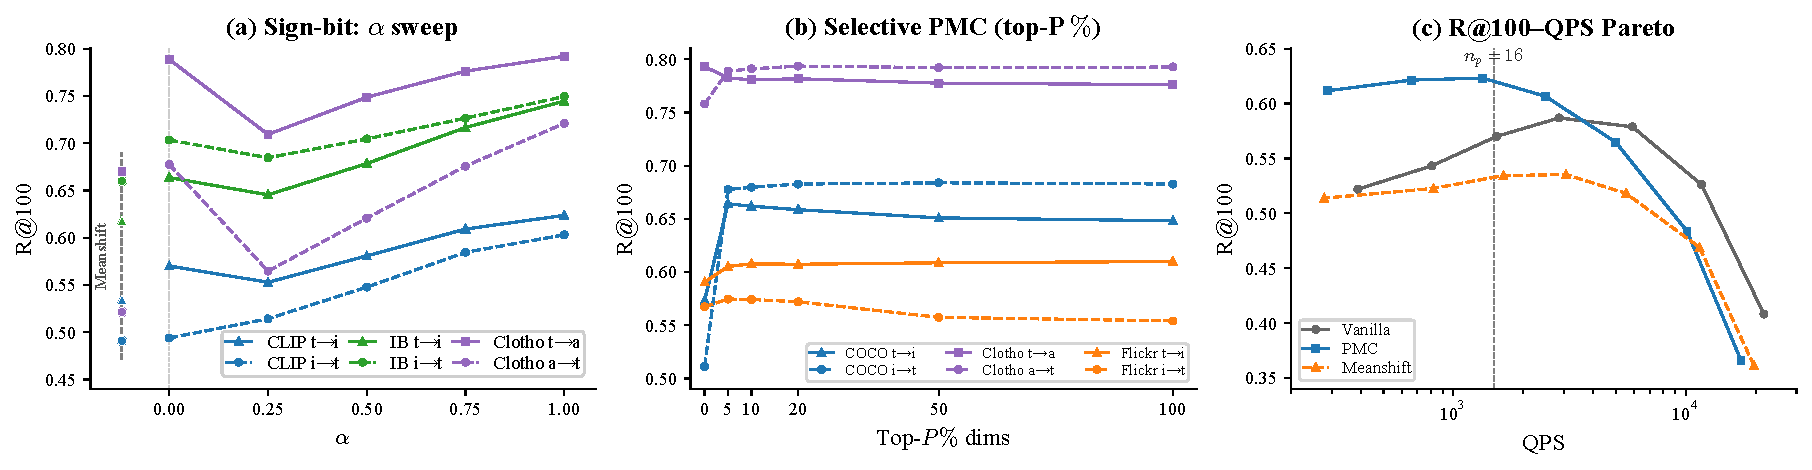
\includegraphics[width=\linewidth]{figures/fig3_analysis.pdf}
  \Description{Three-panel analysis figure. Panel (a) shows BQ alpha sweep curves on MSCOCO and Clotho with mean shift markers and best performance near alpha equals 1. Panel (b) shows selective PMC versus top-P percent dimensions. Panel (c) shows R@100 versus QPS Pareto curves in log-scale where PMC dominates Vanilla at comparable throughput.}
  \caption{(a) BQ R@100 vs.\ shift strength $\alpha$ on MSCOCO+Clotho ($\alpha{=}0$: MeanShift, $\alpha{=}1$: full DB-side PMC): $\alpha{=}1$ is best or near-best, justifying the default. (b) Selective PMC: on concentrated-gap MSCOCO, top-$P{=}5$\% already reaches peak R@100; diffuse gaps require broader correction. (c) R@100--QPS Pareto: PMC dominates Vanilla across throughput levels.}\label{fig:analysis-bcd}
\end{figure*}
